% This file was created by matlab2tikz.
%
%The latest updates can be retrieved from
%  http://www.mathworks.com/matlabcentral/fileexchange/22022-matlab2tikz-matlab2tikz
%where you can also make suggestions and rate matlab2tikz.
%
\definecolor{mycolor1}{rgb}{0.00000,0.44700,0.74100}%
\definecolor{mycolor2}{rgb}{0.85000,0.32500,0.09800}%
%
\begin{figure}[H]
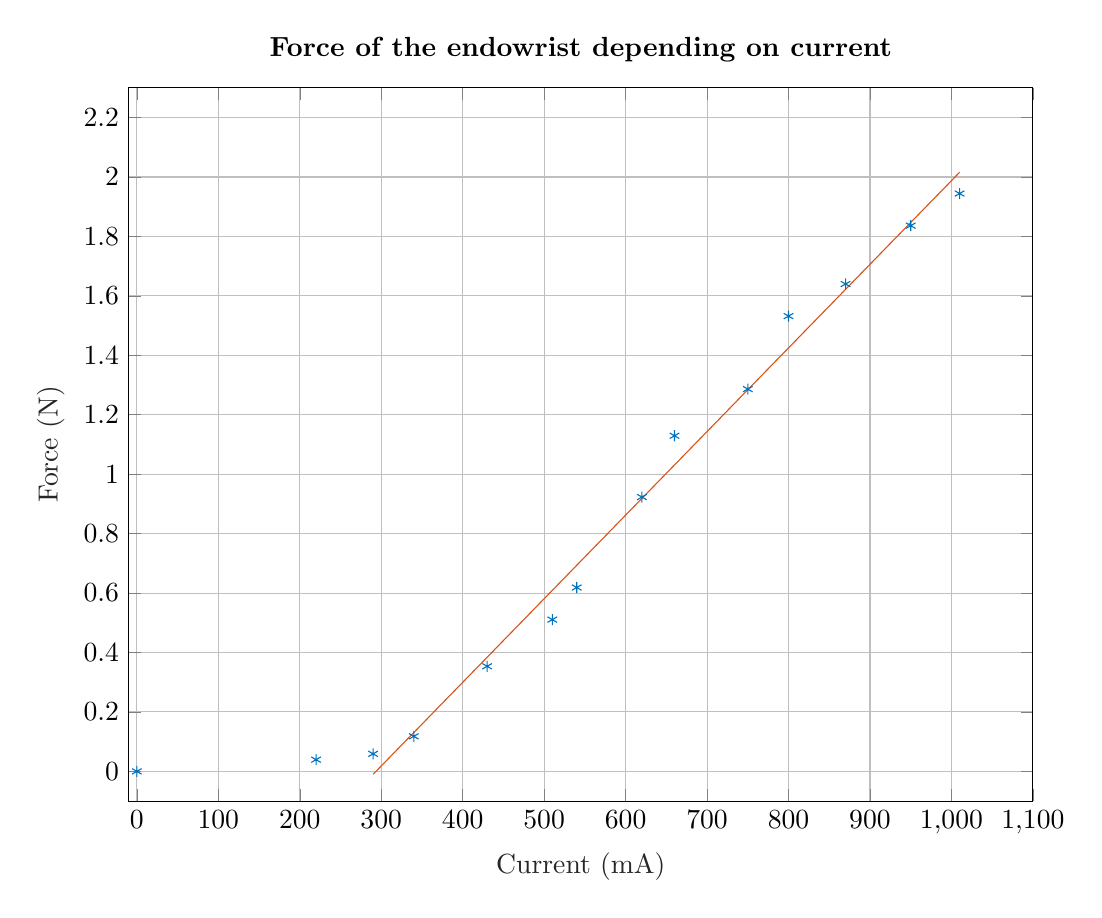
\begin{tikzpicture}

\begin{axis}[%
width=4.521in,
height=3.566in,
at={(0.758in,0.481in)},
scale only axis,
xmin=-10,
xmax=1100,
xlabel style={font=\color{white!15!black}},
xlabel={Current (mA)},
ymin=-0.1,
ymax=2.3,
ylabel style={font=\color{white!15!black}},
ylabel={Force (N)},
axis background/.style={fill=white},
title style={font=\bfseries},
title={Force of the endowrist depending on current},
xmajorgrids,
ymajorgrids
]
\addplot [color=mycolor1, draw=none, mark=asterisk, mark options={solid, mycolor1}, forget plot]
  table[row sep=crcr]{%
0	0\\
220	0.03928\\
290	0.05892\\
340	0.11784\\
430	0.35352\\
510	0.51064\\
540	0.61866\\
620	0.92308\\
660	1.1293\\
750	1.28642\\
800	1.53192\\
870	1.63994\\
950	1.83634\\
1010	1.94436\\
};
\addplot [color=mycolor2, forget plot]
  table[row sep=crcr]{%
290	-0.00996204344902341\\
340	0.130719594329395\\
430	0.383946542330548\\
510	0.609037162776017\\
540	0.693446145443068\\
620	0.918536765888537\\
660	1.03108207611127\\
750	1.28430902411242\\
800	1.42499066189084\\
870	1.62194495478063\\
950	1.8470355752261\\
1010	2.0158535405602\\
};
\end{axis}
\end{tikzpicture}%
\caption{The force measurements from the end-effector with a $0^\circ$ angle.}
\label{endo_force_mes}
\end{figure}